\documentclass{article}
\usepackage{setspace,tikz}
\usepackage[text={6.5in,8.5in},centering]{geometry}
\geometry{verbose,a4paper,tmargin=2.4cm,bmargin=2.4cm,lmargin=2.4cm,rmargin=2.4cm}
\usepackage{graphicx,amsmath,cases,multirow,appendix,graphicx,xcolor}

\setlength\parindent{0pt}

\newcommand{\note}[1]{\colorbox{gray!20}{#1}}
\newcommand{\ind}{\-\hspace{1cm}}
\newcommand*\circled[1]{\tikz[baseline=(char.base)]{
            \node[shape=circle,draw,inner sep=2pt] (char) {#1};}}

\begin{document}


\noindent\makebox[\textwidth][c]{\Large\bfseries  Lecture 4 - Density-independent stochastic growth}

\rule[0.5ex]{\linewidth}{1pt}
\textbf{Announcement}: \\
Hand back Q1\\
Bring laptops next class

\textbf{Today's concepts}: \\
Stochasticity (Environmental vs. Demographic)\\
Expectation vs. Variance (uncertainty)\\
Geometric vs. Arithmetic expectation

\rule[0.5ex]{\linewidth}{1pt}
Review:
Exponential (geometric) as first-order approximation \note{Show examples of population time series}
Discrete vs. continuous \note{Show videos}

\rule[0.5ex]{\linewidth}{1pt}
All previous equations have been deterministic\\
... if we start with same $N(0)$ and $r$ we get exactly the same answer.\\
Add stochasticity:   ``Adding stochastic shell to deterministic core of our model''\\

\textbf{Stochastic} (from the Greek for \emph{aim} or \emph{guess}) = random with respect to considered variables\\
A stochastic process is one whose subsequent state is determined by a random element.
\begin{equation*}
	N_T = N_0 e^{(r\pm noise)T} = N_0 (\lambda \pm noise)^T
\end{equation*}

E.g., 4 years of stochastic growth
\begin{align*}
	N_0 &= 1 &\\
	\lambda_1 &= 2 & N_1 = N_0 \lambda_1 = 1\cdot 2 =  2\\
	\lambda_2 &= 1 & N_2 = N_1 \lambda_2 = 2\cdot 1 =  2\\
	\lambda_3 &= 3 & N_3 = N_2 \lambda_3 = 2\cdot 3 =  6\\
	\lambda_4 &= 2 & N_4 = N_0 \lambda_1 \lambda_2 \lambda_3 \lambda_4 =  12
\end{align*}

\note{Show code in R...}
\begin{center}
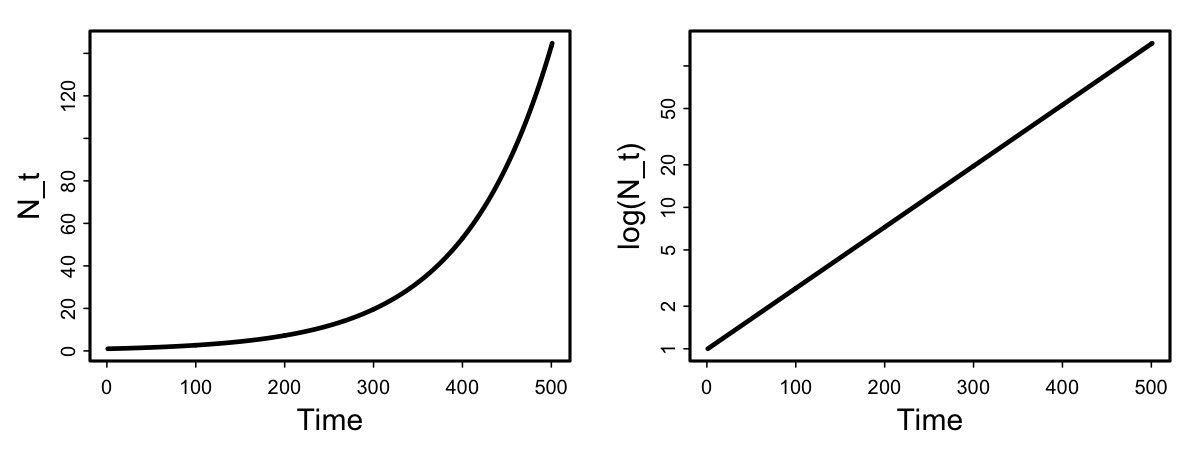
\includegraphics[width=8cm]{figs/image}\\
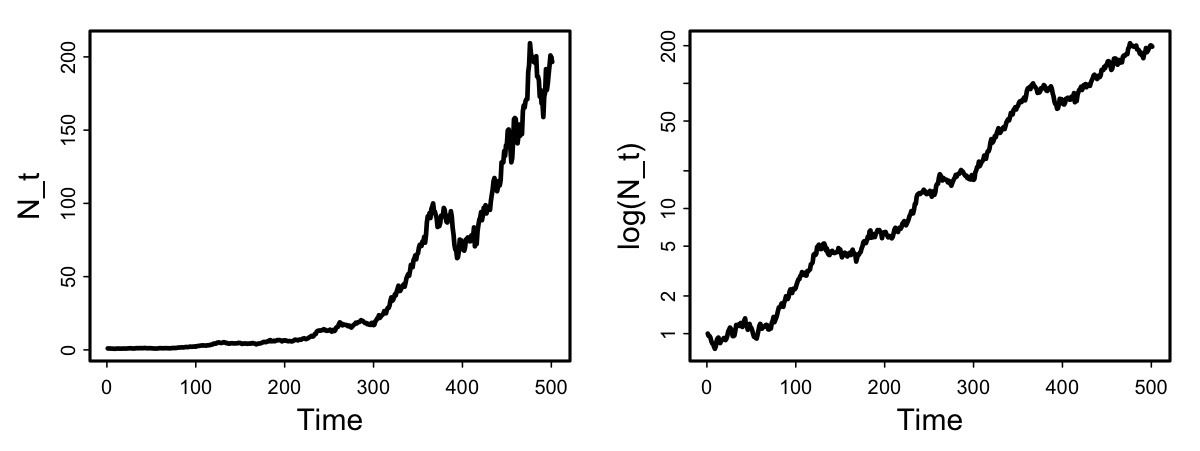
\includegraphics[width=8cm]{figs/image0}
\end{center}

If we wanted to determine:\\
Expectation (mean) of $N_T$ ($\bar{N}_T$) and variance of $N_T$ ($\sigma_{N_T}^2$) \underline{over all time points}:
\begin{align*}
	\bar{N}_T &= E[N_T] = \frac{1}{T}\sum_t^T N_t = \frac{1+2+2+6+12}{5} = 4.6\\
	\sigma_{N_T}^2 & = Var[N_T] =  \frac{1}{T}\sum_t^T (N_t - \bar{N}_T)^2\\
	& = \frac{(1-4.6)^2 + (2-4.6)^2 + (2-4.6)^2 + (6-4.6)^2 + (12-4.6)^2}{5} = 83.2/5 = 16.64
\end{align*}

Note that $\sigma$ = standard deviation\\
\ind and that $CV$ (coefficient of variation) = $\sigma^2/\bar{N}$

\rule[0.5ex]{\linewidth}{1pt}

\pagebreak

\textbf{Environmental Stochasticity} - \emph{temporal variation in population's per capita growth rate}

Importance of distinguishing between geometric vs. arithmetic mean...

Example: Dynamics of two populations with same initial size:
\begin{equation*}
	N(3) = N_0 \lambda_1 \lambda_2 \lambda_3
\end{equation*}
\begin{center}
	Population A: $N_A(3) = N_0 \cdot 2 \cdot 1 \cdot 3 = 6 \cdot N_0$\\
	Population B: $N_B(3) = N_0 \cdot 2 \cdot 2 \cdot 2 = 8 \cdot N_0$
\end{center}

\begin{equation*}
	\bar{\lambda} = \frac{1}{T} \sum_t^T \lambda_t
\end{equation*}
On natural (arithmetic) scale, $\bar{\lambda}_A = \bar{\lambda}_B = 2$.\\

\emph{So why does population $B$ grow more?}\\
Appropriate measure is the geometric mean (remember: popn growth is a multiplicative process):\\
(No standard symbol for geometric mean)

\begin{equation*}
	\text{geometric mean }\lambda = \left(\prod_t^T \lambda_t\right)^{\frac{1}{T}} = \sqrt[T]{\prod_t^T \lambda_t}
\end{equation*}

\begin{center}
	Geometric mean of $\lambda_A = \sqrt[3]{\lambda_1 \cdot \lambda_2 \cdot \lambda_3} = \sqrt[3]{2 \cdot 1 \cdot 3} = 1.817...$\\
	So in fact $N_A(3) = N_0 \cdot 1.817 \cdot 1.817 \cdot 1.817 = 6 \cdot N_0$
\end{center}

\begin{center}\rule[0.1ex]{0.6\linewidth}{1pt}\end{center}
\textbf{Side note: Contrasting arithmetic vs. geometric mean}\\
Two numbers (expressed relative to $x$):
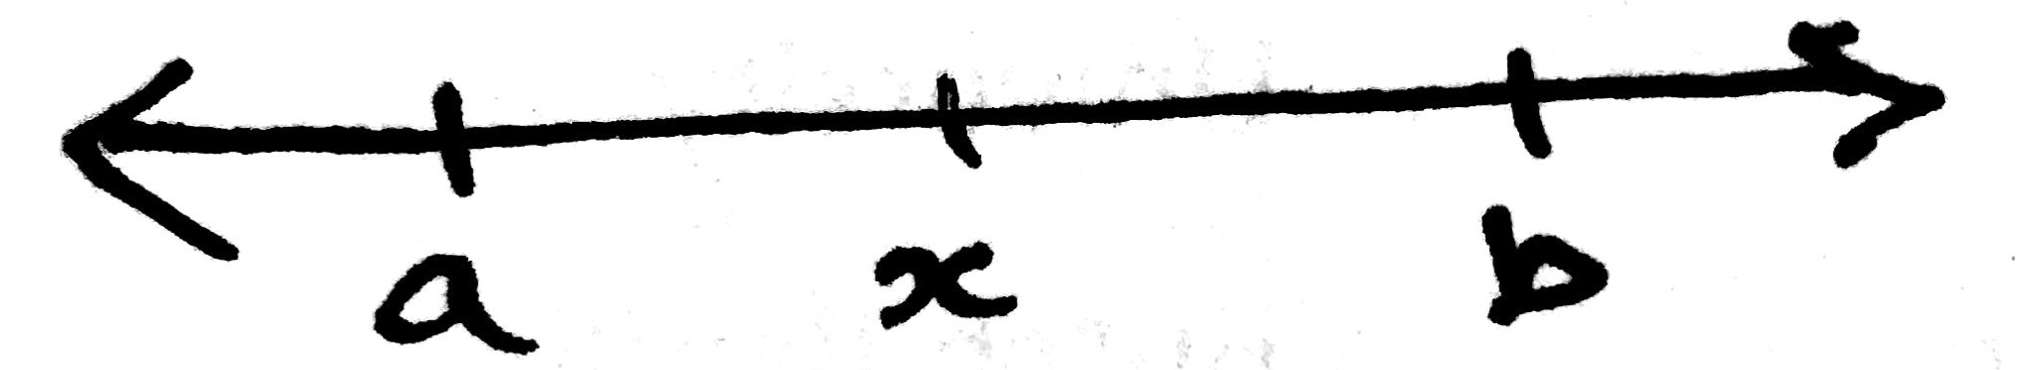
\includegraphics[width=2cm]{figs/ab_line}  What is $x$?
\begin{align*}
	a-x & = x-b & & \frac{a}{x} = \frac{x}{b}\\
	a+b&=2x & & a \cdot b = x \cdot x\\
	\frac{a+b}{2}&=x & & a \cdot b = x^2\\
	&&& \sqrt[2]{a+b} = x
\end{align*}
\begin{center}\rule[0.1ex]{0.6\linewidth}{1pt}\end{center}

Will show that: 	\emph{Natural log of geometric mean $\lambda$ = arithmetic mean of natural log of the $\lambda$'s}
\begin{align*}
	\text{Since...} \ln(b^a) = a\ln(b)  \Rightarrow \quad
	\ln \left( \left(\prod_{t=1}^T \lambda_t \right)^{1/T}\right) &= \frac{1}{T} \cdot \ln(\lambda_1 \cdot \lambda_2 \dots \lambda_T ) \\
	\text{Since...} \ln(ab) = \ln(a)+\ln(b)  \Rightarrow \quad \quad \quad \quad \quad \quad \quad \quad \quad
	&= \frac{1}{T} \left( \ln(\lambda_1) + \ln(\lambda_2) + \dots+ \ln(\lambda_T) \right) \\	
	&=\frac{1}{T} \cdot T \cdot \overline{\ln(\lambda}) \\
	&=\overline{\ln(\lambda)}
\end{align*}
Thus, could also calculate as:
\begin{center}
	Geometric mean $\lambda = e^{\overline{\ln(\lambda)}}$
\end{center}
An alternative approximation (provided in Case, pg. 35):
\begin{center}
	Geometric mean $\lambda = e^{\overline{\ln(\lambda)}} \approx e^{\ln(\bar{\lambda})-\frac{\sigma_\lambda^2}{2\bar{\lambda}^2}}$\\
	(\emph{Note effects of $\sigma_{\lambda}$ and of $\bar{\lambda}$.})
\end{center}
\rule[0.5ex]{\linewidth}{1pt}

\pagebreak

\note{Class R exercise} - random vector draws - compare geometric and arithmetic means 
\begin{itemize}
	\item Effect of $\sigma = 0$, and increasing $\sigma$ values:
		\subitem	Geometric mean will always be less than arithmetic mean 
		\subitem	The more variation, the lower the geometric mean 
	\item	Effect of sample size, $n$:
		 \subitem	Little effect.  very low $n$ might have more variation in depression amount 
	\item	Effect of $\bar{\lambda}$:
		\subitem Raises and lowers, but note that at $\bar{\lambda}\approx 1$, geometric mean $\lambda < 1$  (declining population)!!
\end{itemize}

\textbf{What does this mean for the dynamics of a given focal population}?
\begin{center}
\begin{tabular}{|c|c|c|c|}
\hline \rule[-2ex]{0pt}{5.5ex} \emph{Population change} &  Deterministic $\lambda$ & Deterministic $\ln(\lambda$) &  Environmental noise $\ln(\lambda \pm \text{noise})$\\ 
\hline \rule[-2ex]{0pt}{5.5ex} No change & 1 & 0 & NA \\
\hline \rule[-2ex]{0pt}{5.5ex} Growth  & $>1$ & $>0$  & $\frac{\sigma_\lambda^2}{2\bar{\lambda}^2} <  \ln(\bar{\lambda})>0$  \\ 
\hline \rule[-2ex]{0pt}{5.5ex} Decline & $<1$ & $<0$  & $\ln(\bar{\lambda})-\frac{\sigma_\lambda^2}{2\bar{\lambda}^2}<0$  \\ 
\hline 
\end{tabular}
\end{center} 

\rule[0.5ex]{\linewidth}{1pt}

\textbf{What are the expected mean and variance of $N_T$ for an ``average'' (typical) population?}\\
That is, we will now ask a different question...\\
\ind $\Rightarrow$ What is the expected population size $N_T$ over an ensemble of replicate populations?\\
\ind (The average of $n$ replicate populations.)\\
\note{Run in R...}
\begin{center}
 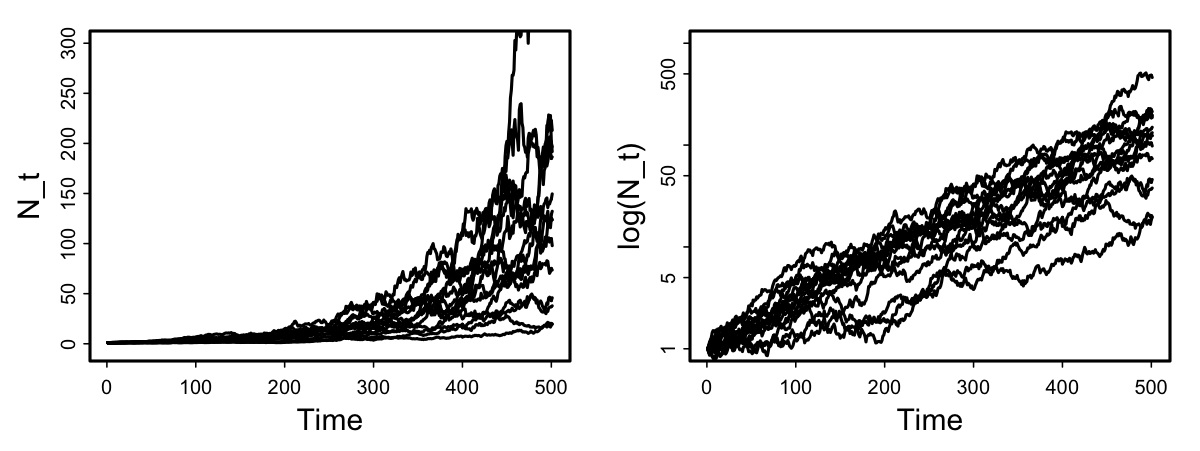
\includegraphics[width=8cm]{figs/image1}\\
 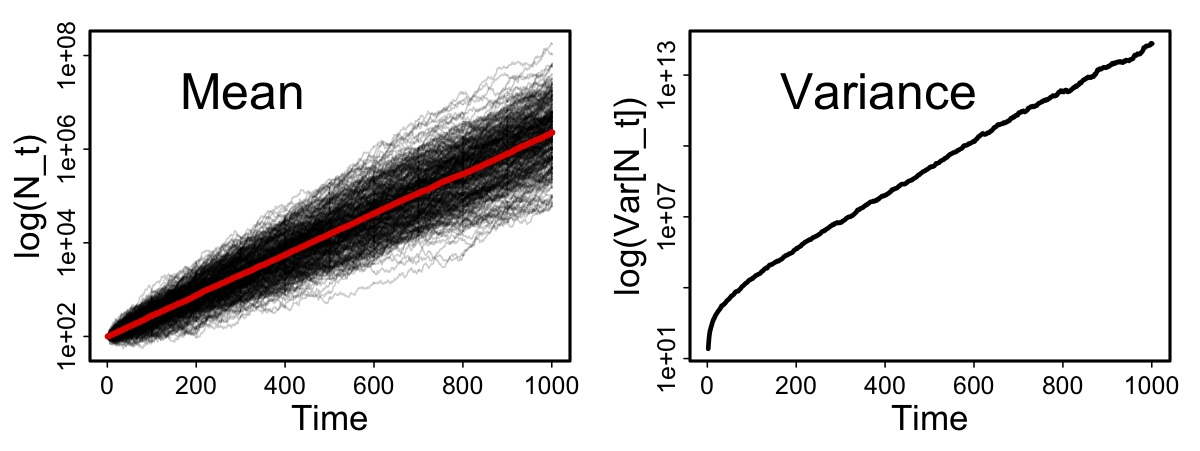
\includegraphics[width=8cm]{figs/image2}
\end{center}

Will show that
\begin{equation*}
	\bar{N}_T = N_0 \bar{\lambda}^T = N_0 e^{\bar{r}t}
\end{equation*}

And that...\\
when there is \emph{environmental variation} only:
\begin{equation*}
	\sigma^2_{ln(N_T)}=T \cdot \sigma^2_{ln(\lambda_t)}
\end{equation*}

when there is only \emph{demographic variation}:
\begin{equation*}
  \sigma_{N_T}^2 =
  \begin{cases} 
        2N_0 \bar{b} T & \text{if } \bar{b}=\bar{d} \\
        \frac{\bar{b}+\bar{d}}{\bar{b}-\bar{d}} N_0 e^{\bar{r}T}(e^{\bar{r}T}-1) & \text{if } \bar{b} \neq \bar{d}
    \end{cases}
 \end{equation*}

\pagebreak

\textbf{How to get $E[N_T]$?}\\
Let $\lambda$ be a random variable from a normal distribution.\\
Any given $\lambda$ from this distribution is denoted by $\lambda_t$.
\begin{align*}
	N_T &= N_0 \prod_{t=1}^T \lambda_t = N_0 \cdot (\lambda_1 \lambda_2 \dots \lambda_T)\\
	E[N_T] &= N_0 \cdot E[\prod_{t=1}^T \lambda_t] \qquad \text{(since } N_0 \text{ is a constant)}\\
		& = N_0 \cdot \prod_{t=1}^TE[\lambda]\\
		& = N_0 \cdot E[\lambda]^T\\
		& = N_0 \cdot \bar{\lambda}^T
\end{align*}

\textbf{How to get variance?}\\
Transform by taking the log...\\
\begin{equation*}
	\ln(N_T)=\ln(N_0)+\ln\left(\prod_{t=1}^T \lambda_t\right) =\ln(N_0)+ \boxed{ \sum_{t=1}^T \ln(\lambda_t)}
\end{equation*}
Now working on the arithmetic scale!\\
Allows us to apply Central Limit Theorem (pg. 41 of Case):
\begin{center}
	\emph{The sum of independent, identically distributed random variables $x_i$ tends to asymptote to the normal density distribution, no matter the underlying distribution of $x_i$}
\end{center}

Under a sufficiently large number of independent random variable draws:
\begin{align*}
	\boxed{\sum_{i=1}^n x_i} & = \mathcal{N}(n\cdot E[x] , \; n\cdot Var[x])\\
	& = \mathcal{N}(n \bar{x}, n \sigma_{x}^2)
\end{align*}

\begin{center}
\emph{The mean of the sum equals the sum of all individual means}\\
\emph{The variance of the sum equals the sum of all individual variances}\\
\end{center}
Inserting $\ln (\lambda_t)$ for $x_i$, we thus have
\begin{align*}
	\sum_{t=1}^T \ln (\lambda_t) & =  \mathcal{N}(T\cdot E[\ln(\lambda_t)] , \; T\cdot Var[\ln(\lambda_t)])\\
	& = \mathcal{N}(T\cdot \overline{\ln(\lambda_t)},\; T\cdot\sigma_{\ln (\lambda_t)}^2)
\end{align*}

Therefore, we have
\begin{equation*}
	E[\ln(N_T)]=\ln(N_0)+ T \cdot \overline{\ln(\lambda_t)}
\end{equation*}
and
\begin{equation*}
\sigma_{\ln (N_T)}^2 = T\cdot \sigma_{\ln(\lambda_t)}^2
\end{equation*}
\\
To translate expectation back to arithmetic scale:\\
Even though the expected value of $N_T$ is $E[N_T]= N_0 \cdot \bar{\lambda}^T$,
\begin{equation*}
	N_T \sim log\mathcal{N} \text{ with median = } e^{\ln(N_0)+T\cdot \overline{\ln(\lambda)}}
\end{equation*}
\\
Take-home message:\\
\textbf{When modeling $N_{t+1}=\lambda N_t$ with environmental noise in growth rate, error must be $log\mathcal{N}$!}\\
\\
In Problem Set \#2 you should therefore use $N_{t+1}=N_t (\lambda \pm e^\epsilon)$, where $\epsilon \sim \mathcal{N}(0,\sigma_\epsilon^2)$.\\

\pagebreak

\textbf{Summary}
\begin{itemize}
\item The solution to $Var[N_T]$ is sensitive to assumed model-formulation!
\item Dependent on how stochasticity is assumed to affect $\lambda$.
\item If you assume $N_{T}=N_0 (\lambda \pm \epsilon)^T$ with $\epsilon \sim \mathcal{N}(0,\sigma_\epsilon^2)$ you'll get a different prediction!
\end{itemize}

\rule[0.5ex]{\linewidth}{1pt}


\textbf{Demographic stochasticity} - Between-individual variation in per capita growth rate\\
Analogy of flipping a coin (not perfect, but will do).
\begin{center}
	$H$ = birth and $T$ = death
\end{center}
\note{Q:} How many $H$ and $T$ in 1000 flips?  How many in 100?  How many in 4?\\
For fair coin, $P(H)=P(T)=0.5$ and $P(H)+P(T)=1 \quad \Rightarrow $ Binomial distribution.

\rule[0.5ex]{\linewidth}{1pt}
\textbf{Class exercise in R}\\
Number of extinctions as function of starting population size using binomial.\\
Going to assume:
\begin{align*}
	P(birth)&=\frac{b}{b+d}\\
	P(death)&=\frac{d}{b+d}
\end{align*}
\begin{center}
	where $b$ and $d$ are per capita birth and death rates, such that $r=b-d$.
\end{center}

\rule[0.5ex]{\linewidth}{1pt}
For true population (no longer binomial):
\begin{align*}
	P(birth)&=\frac{b}{b+d+o}\\
	P(death)&=\frac{d}{b+d+o}\\
	P(other)&=1-[P(b)+P(d)]
\end{align*}
Won't go through derivations, but expectation of $N(t)$ is still:
\begin{equation*}
	\overline{N_t}=N_0 e^{\bar{r}t}
\end{equation*}
But for variance:
\begin{equation*}
  \sigma_{N_T}^2 =
  \begin{cases} 
        2N_0 \bar{b} T & \text{if } \bar{b}=\bar{d} \\
        \frac{\bar{b}+\bar{d}}{\bar{b}-\bar{d}} N_0 e^{\bar{r}T}(e^{\bar{r}T}-1) & \text{if } \bar{b} \neq \bar{d}
    \end{cases}
 \end{equation*}

Side note...Probability of extinction:
\begin{equation*}
	P(ext)=\left(\frac{d}{b}\right)^{N_0}
\end{equation*}

\rule[0.5ex]{\linewidth}{1pt}
Of course, environmental and demographic stochasticity are not mutually exclusive!\\  
Temporal variation among individuals will also causes temporal variation in $\lambda$.\\
See Case for example combining the two.

\rule[0.5ex]{\linewidth}{1pt}
\rule[0.5ex]{\linewidth}{1pt}
\end{document}